\documentclass[12pt]{exam}

% essential packages
\usepackage{fullpage} % margin formatting
\usepackage{enumitem} % configure enumerate and itemize
\usepackage{amsmath, amsfonts, amssymb, mathtools} % math symbols
\usepackage{xcolor, colortbl} % colors, including in tables
\usepackage{makecell} % thicker \Xhline in table
\usepackage{graphicx} % images, resizing

% sometimes needed packages
\usepackage{hyperref} % hyperlinks
% \hypersetup{colorlinks=true, urlcolor=blue}
% \usepackage{logicproof} % natural deduction
\usepackage{tikz} % drawing graphs
\usetikzlibrary{positioning}
% \usepackage{multicol}
% \usepackage{algpseudocode} % pseudocode

% paragraph formatting
\setlength{\parskip}{6pt}
\setlength{\parindent}{0cm}

% newline after Solution:
\renewcommand{\solutiontitle}{\noindent\textbf{Solution:}\par\noindent}

% less space before itemize/enumerate
\setlist{topsep=0pt}

% creates \filcl to grey out cells for groupwork grading
\newcommand{\filcl}{\cellcolor{gray!25}}

% creates \probnum to get the problem number
\newcounter{probnumcount}
\setcounter{probnumcount}{1}
\newcommand{\probnum}{\arabic{probnumcount}. \addtocounter{probnumcount}{1}}

% use roman numerals by default
\setlist[enumerate]{label={(\roman*)}}

% creates custom list environments for grading guidelines, question parts
\newlist{guidelines}{itemize}{1}
\setlist[guidelines]{label={}, left=0pt .. \parindent, nosep}
\newlist{gwguidelines}{enumerate}{1}
\setlist[gwguidelines]{label={(\roman*)}, nosep}
\newlist{qparts}{enumerate}{2}
\setlist[qparts]{label={(\alph*)}}
\newlist{qsubparts}{enumerate}{2}
\setlist[qsubparts]{label={(\roman*)}}
\newlist{stmts}{enumerate}{1}
\setlist[stmts]{label={(\roman*)}, nosep}
\newlist{pflist}{itemize}{4}
\setlist[pflist]{label={$\bullet$}, nosep}
\newlist{enumpflist}{enumerate}{4}
\setlist[enumpflist]{label={(\arabic*)}, nosep}

\printanswers

\begin{document}
%%%%%%%%%%%%%%% TITLE PAGE %%%%%%%%%%%%%%%
\title{EECS 203: Discrete Mathematics\\
  Fall 2023\\
  Homework 6}
\date{}
\author{}
\maketitle
\vspace{-50pt}
\begin{center}
  \huge Due \textbf{Friday, October 20}, 10:00 pm\\
\Large No late homework accepted past midnight.\\
\vspace{10pt}
\large Number of Problems: $5+2$
\hspace{3cm}
Total Points: $100+33$
\end{center}
\vspace{25pt}
\begin{itemize}
    \item \textbf{Match your pages!} Your submission time is when you upload the file, so the time you take to match pages doesn't count against you.
    \item Submit this assignment (and any regrade requests later) on Gradescope. 
    \item Justify your answers and show your work (unless a question says otherwise).
    \item By submitting this homework, you agree that you are in compliance with the Engineering Honor Code and the Course Policies for 203, and that you are submitting your own work.
    \item Check the syllabus for full details.
\end{itemize}
\newpage
%%%%%%%%%%%%%%% TITLE PAGE %%%%%%%%%%%%%%% 

\section*{Individual Portion}
\subsection*{\probnum Set Me Free [18 points]}

\begin{qparts}
    \item For each of the following, determine if the statement is true or false. Justify your answers.
    \begin{qsubparts}
        \item $\emptyset \in \{\{\emptyset\}, \{\emptyset , \{\emptyset\}\}\}$
        \item $\emptyset \subseteq \{\{\emptyset\}, \{\emptyset , \{\emptyset\}\}\}$
        \item $\emptyset \times  \{0,1\} \subseteq \emptyset$
        \item $\{\{1, 2\}\} \subsetneq \{ \{1,2\}, \{2\} \}$
    \end{qsubparts}

    \item Find the cardinality of $\{\emptyset, \emptyset, \{\emptyset, \emptyset\}, \{\emptyset\}\}.$

    \item
        \begin{qsubparts}
        \item Find the cardinality of $\mathcal{P}(\{\emptyset, \{a\}, \{b, c\}\})$.
        \item Find $\mathcal{P}(\{\emptyset, \{a\}, \{b, c\}\})$. Make sure it has the cardinality you wrote in (i).

    \end{qsubparts}

\end{qparts}

\begin{solution}
    \begin{qparts}
        \item 
        \begin{qsubparts}
            \item False.\\
            $\{\{\emptyset\}, \{\emptyset , \{\emptyset\}\}\}$ has only two elements: $\{\emptyset\}$ and $\{ \emptyset, \{ \emptyset\}\}$, $\emptyset$ is not an element.
            \item True.\\
            $\emptyset$ is a subset of every set. So it is also a subset of $\{\{\emptyset\}, \{\emptyset , \{\emptyset\}\}\}$.
            \item True.\\
            The Cartesian product of sets $A$ and $B$ is: $ A \times B = \{ (a,b)| a \in A \land b \in B\}$.\\
            When $A$ is $\emptyset$, $a\in A$ is false for any a. $\therefore$ $a \in A \land b \in B$ is also false.\\
            $\therefore$ there is no such $(a,b)$ that can be an elements of $\emptyset \times B$.\\
            $\therefore \emptyset \times  \{0,1\} = \emptyset$\\ 
            $\because \emptyset \subseteq \emptyset$\\
            $\therefore \emptyset \times \{ 0,1\} \subseteq \emptyset$.   
            \item True.\\
            The only element in $\{\{1, 2\}\}$ is $\{1,2\}$.\\
            And this element is also in $\{ \{1,2\}, \{2\} \}$.\\
            $\therefore \{\{1, 2\}\} \subseteq \{ \{1,2\}, \{2\} \}$.\\
            Notice the element $\{2\}$, $\{2\} \in \{ \{1,2\}, \{2\} \}$, $\{2\} \notin \{\{1, 2\}\}$\\
            $\therefore \{\{1, 2\}\} \subsetneq \{ \{1,2\}, \{2\} \}$.
        \end{qsubparts}
        \item 
        Since the two $\emptyset$ in $\{\emptyset, \emptyset, \{\emptyset, \emptyset\}, \{\emptyset\}\}$ are identical,
        we should remove one to simplify it.\\
        And since the two $\emptyset$ in the element $\{\emptyset, \emptyset\}$ in $\emptyset$ in $\{\emptyset, \{\emptyset, \emptyset\}, \{\emptyset\}\}$
        are identical, we must remove one to simplify it.\\
        After doing that, we have two idential elements $\{ \emptyset\}$ in $\{\emptyset, \{\emptyset\}, \{\emptyset\}\}$, so we must remove one $\{ \emptyset\}$ to simplify it.\\
        $\therefore$ the simplest form of the original set is: $\{\emptyset, \{\emptyset\}\}$.\\
        So the cardinality is $2$ since there are two elements in the set.
        \item 
        \begin{qsubparts}
            \item 
            There are 3 elements in $\{\emptyset, \{a\}, \{b, c\}\}$.\\
            So there are $2^3 =8$ elements in $\mathcal{P}(\{\emptyset, \{a\}, \{b, c\}\})$.\\
            $\therefore$ the cardinality of $\mathcal{P}(\{\emptyset, \{a\}, \{b, c\}\})$ is 8.
            \item 
            $\mathcal{P}(\{\emptyset, \{a\}, \{b, c\}\}) = \{\emptyset, \{\emptyset\}, \{\{a\}\}, \{\{b,c\}\}, \{\{a\}, \{b,c\}\}, \\ \{\emptyset, \{b,c\}\}, \{\emptyset, \{a\}\},  \{\emptyset, \{a\}, \{b,c\}\} \}$.
        \end{qsubparts}
    \end{qparts}
\end{solution}

\subsection*{\probnum Is This Your Card(inality)? [18 points]}
Suppose we define $A = \{m, a, r, c, h\},$ $B = \{ a, r, t, i, c, h, o, k, e\},$ and $C = \{a, e, i, o, u\}.$ Determine the cardinality of each of the following sets. You may leave large exponents unsimplified.

\begin{qparts}
    \item $A \times B$
    \item $\mathcal{P}(A \cup B) $
    \item $\mathcal{P}((A \cap B) \times (B - C))$
\end{qparts}

\begin{solution}
    \begin{qparts}
        \item 
        $\because |A| = 5$, $|B| = 9$,\\
        $\therefore |A \times B| = 5 \times 9 = 45$.
        \item 
        $|A \cup B| = |A| + |B| - |A \cap B|$\\
        $A \cap B = \{a,r,c,h\}, |A \cap B| = 4$\\
        $\therefore |A \cup B| = 5 + 9 - 4 = 10$\\
        $\therefore \mathcal{P}(|A \cup B|) = 2^{10} = 1024$
        \item
        $A \cap B = \{a,r,c,h\}$,\\
        $B - C = \{r,t,c,h,k\}$, \\
        $\therefore |(A \cap B) \times (B - C)| = 4 \times 5 = 20$.\\
        $\therefore |\mathcal{P}((A \cap B) \times (B - C))| = 2^{20} = 1024 \times 1024 = 1048576$
    \end{qparts}
\end{solution}

\subsection*{\probnum Ice Cream Truck! [20 points]} 
There are 40 IAs for EECS 203 and they are all waiting in line for the ice cream truck! At the ice cream truck, every IA orders at least one flavor of ice cream, but they have the option to order more.
\begin{itemize}
    \item 22 of them ordered chocolate ice cream
    \item 25 of them ordered strawberry ice cream
    \item 16 of them ordered vanilla ice cream
\end{itemize}
These numbers add up to more than 40, so we know that some IAs must have ordered multiple flavors. We also know:
\begin{itemize}
    \item 12 IAs ordered chocolate ice cream and strawberry ice cream,
    \item 8 ordered strawberry ice cream and vanilla ice cream,
    \item 10 ordered vanilla cream and chocolate ice cream,
    \item and of these, some IAs ordered all three.
\end{itemize}
How many IAs ordered all three flavors? Show all your calculations.

\textbf{Note:} A Venn diagram is not acceptable justification for this question.

\begin{solution}
    We use $A$ to represent the set of IAs who ordered chocolate ice cream;\\
    and $B$: the set of IAs who ordered strawberry ice cream;\\
    and $C$: the set of IAs who ordered vanilla ice cream;\\
    Then the given information is that: \\
    Above all, $|A \cup B \cup C| = 40$.\\
    And $|A| = 22 ,|B| = 25 , |C| = 16$.\\
    And $|A \cap B| = 12, |B \cap C| = 8, |A \cap C| = 10$.\\
    Since $|A \cup B \cup C| = |A| + |B| + |C| - |A \cap B| - |A \cap C| - |B \cap C| + |A \cap B \cap C|$,\\
    $|A \cap B \cap C| = |A \cup B \cup C| - |A| - |B| - |C| + |A \cap B| + |A \cap C| + |B \cap C| = 40 - 22 - 25 - 16 + 12 + 8 + 10 = 7$

\end{solution}

\subsection*{\probnum S$\cup$bset Fu$\cap$ [20 points]}
Let $A$, $B$, and $C$ be sets. Prove that $$(B - A) \cup (C - A) = (B \cup C) - A$$
by showing that each is a subset of the other. 

\begin{solution}
    \begin{qparts}
        \item We prove that $(B - A) \cup (C - A) \subseteq ((B \cup C) - A)$, that is, any element in $(B - A) \cup (C - A)$ is also in $(B \cup C) - A$.\\
        Let $x$ be an arbitrary element in the domain.\\
        If $x \ in (B - A) \cup (C-A)$, $x \in (B-A) \lor x \in (C-A)$ due to definition of set union.\\
        $\therefore (x \in B \land x \notin A) \lor (x \in C \land x \notin A)$ due to definition of set substraction.\\
        $\therefore (x \in B \land \lnot x \in A) \lor (x \in C \land \lnot x \in A)$\\
        $\therefore \lnot x \in A \land (x \in B \lor x \in C)$ due to distributive law.\\
        $\therefore (x \in B \cup C) \land (x \notin A)$\\
        $\therefore x \in ((B \cap C) - A)$ due to definition of set union.\\
        $\therefore (B - A) \cup (C - A) \subseteq ((B \cup C) - A)$ due to definition of subset.
        \item We prove that $((B \cup C) - A) \subseteq (B - A) \cup (C - A)$, that is, any element in $(B \cup C) - A$ is also in $(B - A) \cup (C - A)$.\\
        Let $x$ be an arbitrary element in the domain.\\
        If $x \in ((B \cup C) - A)$, ($x \in (B \cup C)) \land (x \notin A)$ due to definition of set substraction.\\
        $\therefore ((x \in B) \lor (x \in C)) \land (\lnot x \in A)$ due to definition of set union.\\
        $\therefore (x \in B \land \lnot x \in A) \lor (x \in C \land \lnot x \in A)$ due to distributive law.\\
        $\therefore (x \in (B - A)) \lor (x \in (C - A))$ due to definition of set substraction.\\
        $\therefore ((B \cup C) - A) \subseteq (B - A) \cup (C - A)$ due to definition of subset.
    \end{qparts}
    Since $(B - A) \cup (C - A) \subseteq ((B \cup C) - A)$ and $((B \cup C) - A) \subseteq (B - A) \cup (C - A)$, 
    \\ $(B - A) \cup (C - A) = (B \cup C) - A$.
\end{solution}


\subsection*{\probnum Subset Size Question [24 points]}
Given that $A, B, C$ are sets with $|A| = 13$, $|B| = 8$, $|C| = 10$, find the maximum \textit{and} the minimum possible cardinalities of the following sets in the domain of integers.\\

\begin{qparts}
    \item $\overline{A} \cap B$   
    \item $A \cap (B \cup C)$
    \item $\mathcal{P}(B \times C)$
    \item $(A - B) \cap C$
\end{qparts}
\begin{solution}
    \begin{qparts}
        \item 
        Due to intersection, $|\overline{A} \cap B| \leq |B| = 8$\\
        Since a set cannot have fewer than 0 element, $|\overline{A} \cap B| \geq 0$.\\
        When $A \cap B = \emptyset$, then $\overline{A} \cap B = B$, then $|\overline{A} \cap B| = |B| = 8$.\\
        When $B \subseteq A, A \cap B = B$, then $\overline{A} \cap B = \emptyset$, then $|\overline{A} \cap B| = |\emptyset| = 0$.\\
        $\because$ These two situations are all possible, \\
        $\therefore$ the maximum possible cardinality is 8, and the minimum cardinality of $\overline{A} \cap B$ is 0.
        \item 
        Due to union, $|B \cup C| \geq max(|B|,|C|) = 10$ and $|B \cup C| \leq |B| + |C| = 18$.\\
        Due to intersection, $|A \cap (B \cup C)| \geq 0$ and $|A \cap (B \cup C)| \leq min(|A|, |B \cup C|)$.\\
        $\because |A| = 13, 10 \leq |B \cup C| \leq 18$,\\
        When $10 \leq |B \cup C| < 13$, $min(|A|,|B \cup C|) = |B \cup C| < 13$;\\
        When $13 \leq |B \cup C| \leq 18$,  $min(|A|,|B \cup C|) = |A| = 13$.\\
        $\therefore$ the maximum value of $|A \cap (B \cup C)|$ is 13.\\
        $\therefore$ The minimum possible cardinality is 0 and maximum possible cardinality is 13.
        \item 
        Since $|B| = 8, |C| = 10$, $B,C$ cannot be $\emptyset$. \\
        $\therefore$ $|B \times C|$ can only be $|B| \times |C| = 80$. 
        \\$\therefore$ $|\mathcal{P}(B \times C)|$ can only be $2^{|B \times C} = 2^80$
        \\$\therefore$ The maximum possible cardinality and the minimum possible cardinality are both $2^{80}$.
        \item 
        Due to substraction, $|A| - |B| \leq |A- B| \leq |A|$.\\
        $\therefore 5 \leq |A-B| \leq 13$.\\
        Due to intersection, $0 \leq |(A-B) \cap C| \leq min(|A-B|, |C|)$\\
        When $|A - B| <10$, $min(|A-B|, |C|) = |A-B| < 10$. When $|A-B| \geq 10$,  $min(|A-B|, |C|) = |C| = 10$. 
        \\$\therefore $ the overall range is $0 \leq |(A-B) \cap C| \leq 10$.
        \\$\therefore$ the maximum possible cardinality is 10 and the minimum possible cardinality is 0.

    \end{qparts}
\end{solution}

\pagebreak
\setcounter{probnumcount}{1}
\section*{Groupwork}
\subsection*{\probnum Grade Groupwork 5}
Using the solutions and Grading Guidelines, grade your Groupwork 5:
\begin{itemize}
    \item Mark up your past groupwork and submit it with this one.
    \item Write whether your submission achieved each rubric item. If it didn't achieve one, say why not.
    \item Use the table below to calculate scores.
    \item For extra credit, write positive comment(s) about your work.
    \item You don't have to redo problems correctly, but it is recommended!
    \item What if my group changed? \begin{itemize}
        \item If your current group submitted the same groupwork last time, grade it together.
        \item  If not, grade your version, which means submitting this groupwork assignment separately. You may discuss grading together.
    \end{itemize}
\end{itemize}

\begin{center}
\resizebox{\textwidth}{!}{\begin{tabular}{| c | c | c | c | c | c | c | c | c | c | c | c | c |}
\hline
 & (i) & (ii) & (iii) & (iv) & (v) & (vi) & (vii) & (viii) & (ix) & (x) & (xi) & Total:\\
\hline
Problem 2 & & & & \filcl & \filcl &\filcl &\filcl &\filcl &\filcl & \filcl& \filcl& \hspace{1cm}/12\\
\hline 
Problem 3 & & & & & & \filcl & \filcl &\filcl &\filcl & \filcl& \filcl& \hspace{1cm}/8\\
\Xhline{1.25pt}
Total: &\filcl &\filcl &\filcl &\filcl &\filcl &\filcl &\filcl &\filcl & \filcl& \filcl& \filcl&\hspace{1cm}/20\\
\hline
\end{tabular}}
\end{center}

\subsection*{Previous Groupwork 5(1): Polly Gone [12 points]}

A convex polygon is a 2D shape with all straight edges such that any line segment between any two non-adjacent vertices passes entirely through its interior (see example picture below). Show via induction that the sum of the interior angles of a convex polygon with $n$ sides is $(n - 2) \cdot 180^{\circ}$. Don't include unneeded base cases.

\begin{center}
    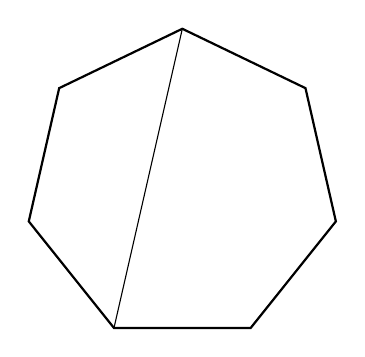
\begin{tikzpicture}[scale = 2]
        \draw[thick, black]  (0,1) -- (0.782,0.623) -- (0.975,-0.223)--(0.434,-0.9)--(-0.434,-0.9)--(-0.975,-0.223)--(-0.782,0.623)--cycle;
        \draw[thin,black] (0,1) -- (-0.434,-0.9);
    \end{tikzpicture}
\end{center}

\textbf{Hint 1}: It is helpful to know that a triangle's interior angles always sum to $180^{\circ}$. You may assume this is true for the problem.

\textbf{Hint 2}: In order to apply your inductive hypothesis to a convex polygon, you'll need to think of it in terms of smaller convex polygons. How can you make smaller polygons out of a big one?

\begin{solution}
    Let $k(n)$ = the sum of the interior angles of a convex polygon with $n$ sides\\
    $P(n): k(n) = (n-2) \cdot 180^{\circ} $\\
    Let $K$ be an arbitrary integer in the domain that $k \geq 4$.\\
    Assume: $P(3) \land P(4) \land P(5) \land ... \land P(k-1)$\\
    Want to prove: $P(k)$
    \\\\
    \textbf{Base Case:}\\
    (Triangle) $n=3$, the sum of the interior angles is $180^\circ $\\
    $k(3) = (3-2) \times 180^\circ  = 1 \times 180^\circ  = 180^\circ $.
    \\\\
    \textbf{Inductive Step:}\\
    Use a straight line to divide the $k$-sides polygon into a triangle and a $(k-1)$-sides polygon.\\
    Using the inductive assumption we know that the $k$-sided polygan should have $(k-2) \times 180^\circ $ degrees for its interior angles.

    Tus the sum of the interior angles is 
    \begin{align*}
        180^\circ  + (k-1-2) \times 180^\circ &= 180^\circ  + (k-3) \times 180^\circ 
                                              &= 180^\circ  \times (1 + k - 3) 
                                              &= 180(k-2)^\circ 
    \end{align*}

    Therefore $P(k)$ is true for every integer $k \geq 4$.
\end{solution}


\smallskip
\subsection*{Previous Groupwork 5(2): Running Recurrence [8 points]}
An EECS 203 student goes to lecture everyday. On each day, she always chooses exactly one method of transportation, and always chooses to walk, bike, or take a bus. She also follows additional rules:
\begin{itemize}
    \item She never walks two days in a row.
    \item If she takes the bus, she must have biked two days ago and walked a day ago.
\end{itemize}

Let $a_n$ denote the number of ways she can go to EECS 203 lecture across $n$ days for $n \geq 0$.
\begin{qparts}
    \item Find a recurrence relation for $a_n$.
    \item What are the initial conditions? Use the fewest initial conditions necessary.
\end{qparts}

\begin{solution}
    \begin{qparts}
        \item The recurrence relation is:
            $$
            a_n = a_{n-1} + a_{n-2} + a_{n-3} + a_{n-4}
            $$
            \begin{center}
                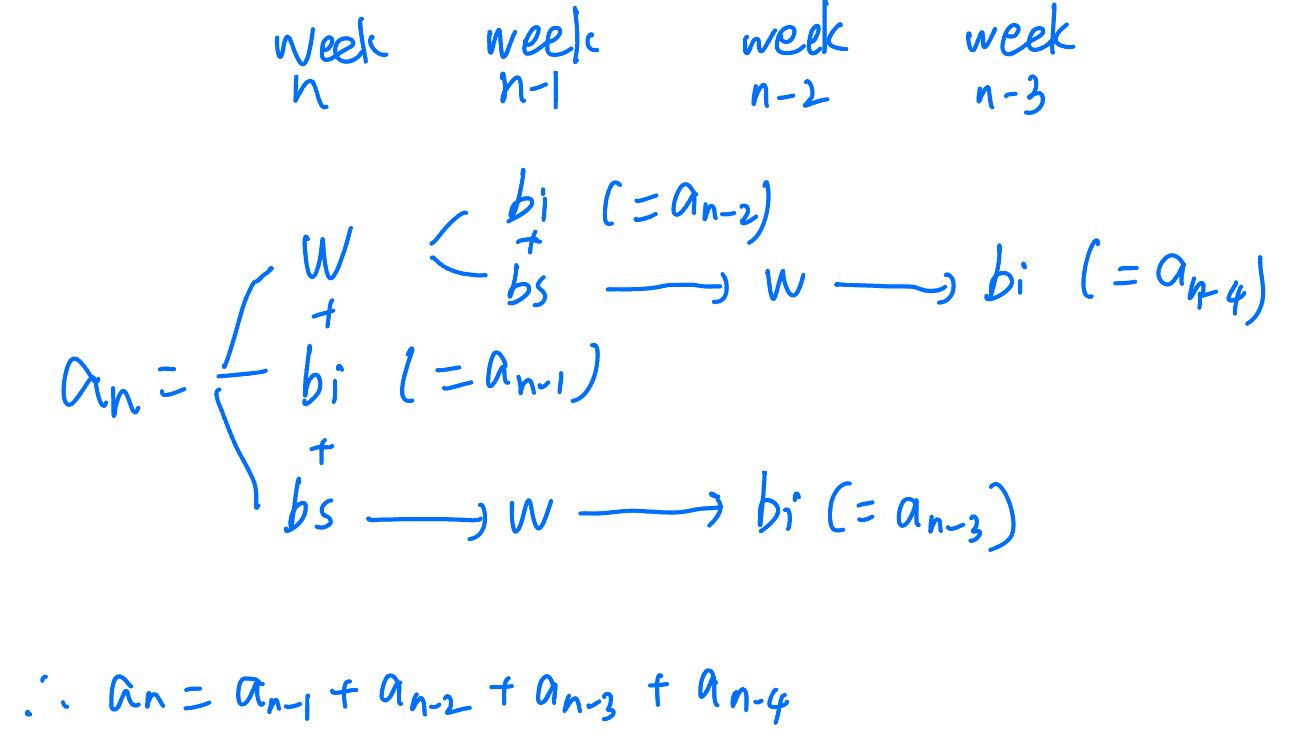
\includegraphics[scale=0.2]{4.jpg}
            \end{center}

            There are 3 cases for the week $n$.\\

            Case 1: In week $n$, she goes to school by bike. This choice has no restrction, so in the weeks before,
            the number of ways she could go to lecture is $a_{n-1}$.
            \\Case 2: In week $n$, she goes to school by bus. This means that in week $n-1$, she walked to school and in
            week $n-2$, she went to lecture by bike. In the weeks before, the number of ways she could go to lecture is $a_{n-3}$.\\
            Case 3: In week $n$, she walks to school. This means that in week $n-1$, she can only went to lecture by bike or by bus. In the
            case she went to lecture by bike, the number of ways she could go to lecture before is $a_{n-2}$. And in the case she wen to 
            lecture by bus, we apply the same logic as in case 2 and get that before the week, the number of ways she could 
            go to lecture is $a_{n-4}$.
        \item
            Since for $a_n$, $n \geq 0$, and in our recurrence relation there is $a_{n-4}$. We need $n-4 \geq 0$ for the 
            recurrence relation. So the cases where $0 \leq n < 4$ should be initial conditions.\\
            That is:
            \\ $a_0 = 1$ (no way)
            \\ $a_1 = 2$ (can only go by bike or on foot)
            \\ $a_2 = 3$ (walk bike, bike walk, bike bike)
            \\ $a_3 = 6$ (walk bike walk, walk bike bike, bike bike walk, bike walk bike, bike bike bike, bike walk bus)

    \end{qparts}
\end{solution}


\subsection*{\probnum (Set)ting up a (Power)ful Proof [17 points]}
\begin{qparts}
    \item Suppose we want to prove by Induction that for any finite set $S$, it is true that $|\mathcal{P}(S)| = 2^{|S|}$. What is the Inductive Hypothesis for your proof? \emph{Hint: Consider what variable you should do induction on.}
    \item Prove by Induction that for any finite set $S$, it is true that $|\mathcal{P}(S)| = 2^{|S|}$.
\end{qparts}
\begin{solution}

\end{solution}

\subsection*{\probnum Out of the ordinary [16 points]}
The (von Neumann) ordinals are a special kind of number. Each one is represented just in terms of sets. We can think of every natural number as an ordinal. We won't deal with it in this question, but there are also infinite ordinals that ``keep going" after the natural numbers, which works because there are infinite sets.

The smallest ordinal, $0$, is represented as $\emptyset$. Each ordinal after is represented as the set of all smaller ordinals. For example,
\begin{align*}
    0 &= \emptyset\\
    1 &= \{ 0 \} = \{ \emptyset \}\\
    2 &= \{ 0, 1 \} = \{ \emptyset, \{ \emptyset \} \}\\
    3 &= \{ 0, 1, 2 \} = \{ \emptyset, \{ \emptyset \}, \{ \emptyset, \{ \emptyset \} \} \}
\end{align*}

\begin{qparts}
    \item What is the ordinal representation of $4$, in terms of just sets?

    \item If the sets $X$ and $Y$ are ordinals representing the natural numbers $x$ and $y$ respectively, how can we tell if $x \le y$ in terms of $X$ and $Y$? Why does this work?

    \item If $X$ is the ordinal representing the natural number $x$, what is the ordinal representation of $x+1$? Why does this work?
\end{qparts}

\begin{solution}

\end{solution}

\end{document}